\chapter{Model Overview}

In this chapter, I will discuss two generative models in the order of their development: Variational Autoencoders (VAEs) and Diffusion Models. These models represent key milestones in the evolution of generative modeling techniques.

\section{Variational Autoencoders (VAEs)}

Variational Autoencoders (VAEs) were introduced in 2013 and are one of the earliest forms of generative models. VAEs aim to model the underlying distribution of data by learning a compressed representation, or latent vector, \(z\), of the input data \(x\).

The VAE architecture consists of two main components, as shown in Figure~\ref{fig:VAE_structure}:
\begin{itemize}
  \item \textbf{Encoder} \( q_\phi(z|x) \): The encoder compresses the input data \(x\) into a latent vector \(z\). The encoder is parameterized by \(\phi\), which represents the parameters of the encoding neural network.
  \item \textbf{Decoder} \( p_\theta(x|z) \): The decoder takes the latent vector \(z\) and attempts to reconstruct the original data \(x'\) that resembles the input \(x\). The decoder is parameterized by \(\theta\), representing the parameters of the decoding neural network.
\end{itemize}

\begin{figure}[h]
    \centering
    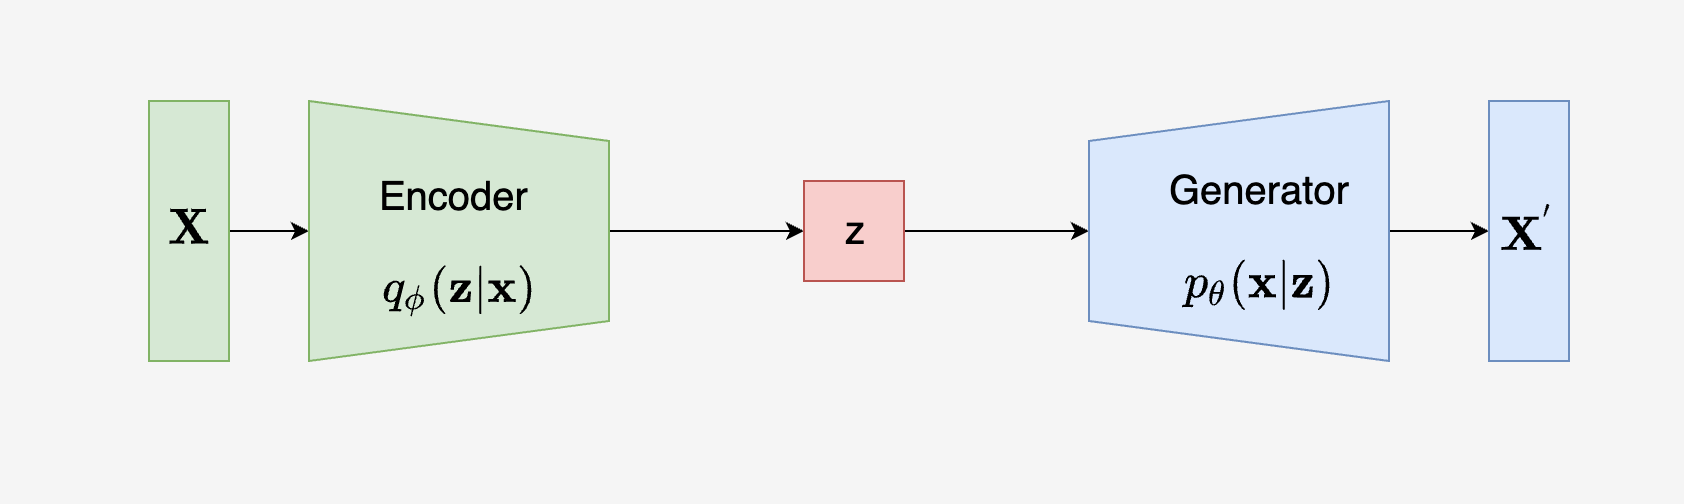
\includegraphics[width=0.9\textwidth]{./Images/VAE_structure.jpg}
    \caption{VAE structure showing the encoder and decoder processes.}
    \label{fig:VAE_structure}
\end{figure}

The training objective of VAEs is to maximize the \textit{variational lower bound}, which involves balancing two terms: the reconstruction error and the regularization term (Kullback-Leibler divergence). This ensures that the model learns meaningful latent representations that allow it to generate new data.

The loss function for VAE is defined as:

\begin{equation}
\mathcal{L} = \mathbb{E}_{q_\phi(z|x)}[\log p_\theta(x|z)] - D_{KL}(q_\phi(z|x) \| p(z))
\end{equation}

Where:
\begin{itemize}
    \item \(\mathcal{L}\): The total loss that the model aims to minimize.
    \item \(\mathbb{E}_{q_\phi(z|x)}[\log p_\theta(x|z)]\): The expected log-likelihood of reconstructing the data \(x'\) from the latent variable \(z\). The distribution \(q_\phi(z|x)\) represents the encoder, while \(p_\theta(x|z)\) represents the decoder's attempt to reconstruct the input data.
    \item \(D_{KL}(q_\phi(z|x) \| p(z))\): The Kullback-Leibler (KL) divergence, which measures the difference between the encoder's latent distribution \(q_\phi(z|x)\) and the prior distribution \(p(z)\), typically assumed to be Gaussian.
\end{itemize}

Visualizing the Process:

1. Encoding Step: The input data \(x\) is passed through the encoder, which compresses it into the latent representation \(z\). This process is modeled by the distribution \(q_\phi(z|x)\), as seen on the left side of Figure~\ref{fig:VAE_structure}.

2. Latent Representation: The latent variable \(z\) is sampled from the encoder's distribution. It serves as a more compact representation of the original data.

3. Decoding Step: The decoder \(p_\theta(x|z)\) takes the latent representation \(z\) and attempts to reconstruct the original data \(x'\), as seen on the right side of the figure.

In simple terms, the encoder learns to compress the data into a lower-dimensional space, while the decoder learns to reconstruct the original data from this compact representation. VAEs are commonly used in tasks such as image generation, where the goal is to create new images that resemble the input data.



\section{Diffusion Models}

Diffusion models are the most recent advancement in generative models, first introduced in the early 2020s. These models take a different approach by progressively adding noise to data and then learning to reverse the process, effectively "denoising" the noisy data back into its original form.

The process involves two key steps, as shown in Figure~\ref{fig:Diffusion_structure}:
\begin{itemize}
  \item \textbf{Forward Process}: Gradually adds Gaussian noise to data \(x_0\), creating noisy versions of the data \(x_1, x_2, \dots, x_T\). Each step increases the level of noise, eventually leading to a completely noisy version \(z\).
  \item \textbf{Reverse Process}: The model learns to reverse the noise addition process, starting from the fully noisy version \(z\), and progressively denoising it to recover data that resembles the original input \(x_0\).
\end{itemize}

\begin{figure}[h]
    \centering
    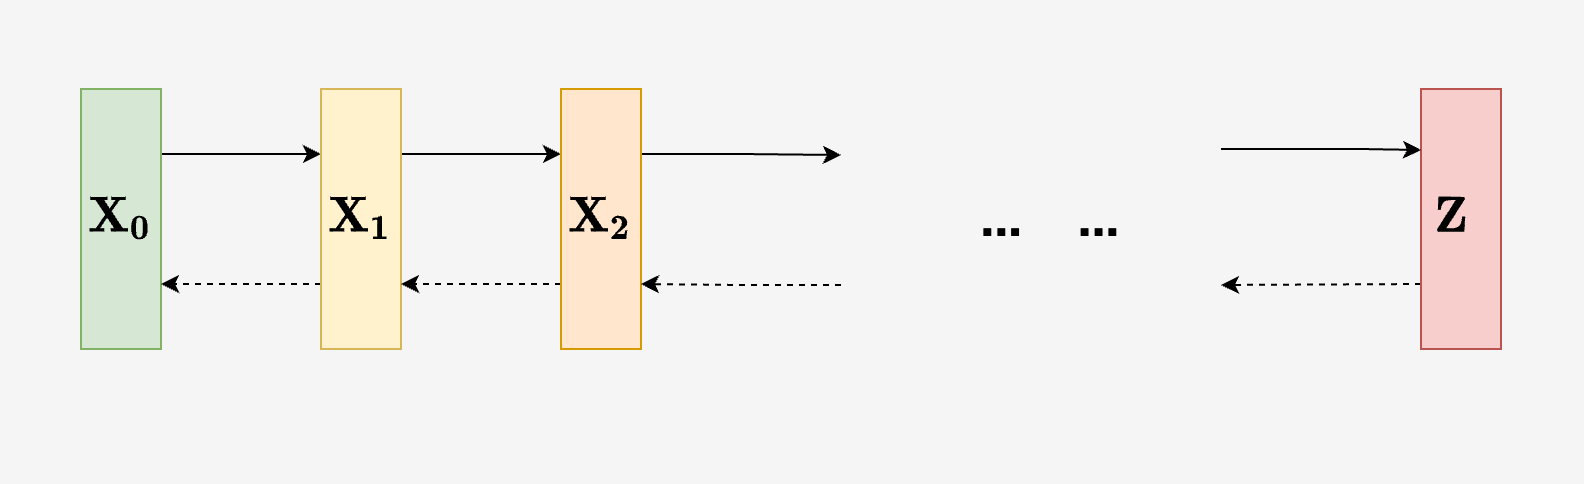
\includegraphics[width=0.9\textwidth]{./Images/Disffusion_structure.jpg}
    \caption{Diffusion model structure showing the forward and reverse processes.}
    \label{fig:Diffusion_structure}
\end{figure}

Forward Process:
In the forward process, starting from the original data \(x_0\), Gaussian noise is added step-by-step to generate increasingly noisy versions of the data. Mathematically, the forward process is described as:

\begin{equation}
q(x_t | x_{t-1}) = \mathcal{N}(x_t; \sqrt{\alpha_t} x_{t-1}, \beta_t I)
\end{equation}

Where:
\begin{itemize}
    \item \(x_0\), \(x_1\), \(x_2\), \dots, \(x_T\): The sequence of noisy data at each time step.
    \item \(\alpha_t\): The scaling factor applied to the data at each step.
    \item \(\beta_t\): The variance of the Gaussian noise added at each step \(t\).
    \item \(\mathcal{N}(x; \mu, \sigma^2)\): A Gaussian distribution with mean \(\mu\) and variance \(\sigma^2\).
\end{itemize}

The process continues until we reach the final state \(z\), which is almost entirely noise.

Reverse Process:
Once the noisy data is generated, the reverse process begins. The model learns to reverse the noise addition process to gradually recover the original data. The reverse process is defined as:

\begin{equation}
p_\theta(x_{t-1} | x_t) = \mathcal{N}(x_{t-1}; \mu_\theta(x_t, t), \Sigma_\theta(x_t, t))
\end{equation}

Where:
\begin{itemize}
    \item \(x_t\): The noisy data at time step \(t\).
    \item \(\mu_\theta(x_t, t)\): The model's predicted mean at step \(t\), parameterized by \(\theta\).
    \item \(\Sigma_\theta(x_t, t)\): The model's predicted variance at step \(t\), parameterized by \(\theta\).
    \item \(\mathcal{N}(x; \mu, \sigma^2)\): A Gaussian distribution with mean \(\mu\) and variance \(\sigma^2\).
\end{itemize}

The reverse process progressively reduces the noise added in the forward process, resulting in data that closely resembles the original input.

Loss Function:
The training objective for diffusion models is to minimize the difference between the real data distribution and the distribution of generated data across all time steps:

\begin{equation}
L = \sum_{t=1}^{T} \mathbb{E}_{x_0, \epsilon} [\|\epsilon - \epsilon_\theta(x_t, t)\|^2]
\end{equation}

Where:
\begin{itemize}
    \item \(L\): The loss function to be minimized.
    \item \(T\): The total number of time steps in the diffusion process.
    \item \(x_0\): The original data sample.
    \item \(x_t\): The data at time step \(t\), after adding noise.
    \item \(\epsilon\): The noise added to the data at each step.
    \item \(\epsilon_\theta(x_t, t)\): The model's estimate of the noise at time step \(t\).
\end{itemize}

Visualizing the Process:

1. Forward Process: As shown in Figure~\ref{fig:Diffusion_structure}, the original data \(x_0\) is progressively corrupted by adding noise step-by-step to generate noisy versions \(x_1, x_2\), and so on, until reaching \(z\), which is almost pure noise.

2. Reverse Process: The reverse process starts with the noisy data \(z\) and progressively removes noise to reconstruct the original data \(x_0\).

This iterative denoising approach has proven effective in generating photorealistic images and other complex data types. Diffusion models are particularly stable to train, and their ability to generate high-quality samples has made them a powerful tool in generative modeling.